\documentclass{beamer}
\usepackage[utf8]{inputenc}

\usetheme{Madrid}
\usecolortheme{default}
\usepackage{amsmath,amssymb,amsfonts,amsthm}
\usepackage{txfonts}
\usepackage{tkz-euclide}
\usepackage{listings}
\usepackage{adjustbox}
\usepackage{array}
\usepackage{tabularx}
\usepackage{gvv}
\usepackage{lmodern}
\usepackage{circuitikz}
\usepackage{tikz}
\usepackage{graphicx}
\usepackage{multicol}

\setbeamertemplate{page number in head/foot}[totalframenumber]

\usepackage{tcolorbox}
\tcbuselibrary{minted,breakable,xparse,skins}

\definecolor{bg}{gray}{0.95}
\DeclareTCBListing{mintedbox}{O{}m!O{}}{%
  breakable=true,
  listing engine=minted,
  listing only,
  minted language=#2,
  minted style=default,
  minted options={%
    linenos,
    gobble=0,
    breaklines=true,
    breakafter=,,
    fontsize=\small,
    numbersep=8pt,
    #1},
  boxsep=0pt,
  left skip=0pt,
  right skip=0pt,
  left=25pt,
  right=0pt,
  top=3pt,
  bottom=3pt,
  arc=5pt,
  leftrule=0pt,
  rightrule=0pt,
  bottomrule=2pt,
  toprule=2pt,
  colback=bg,
  colframe=orange!70,
  enhanced,
  overlay={%
    \begin{tcbclipinterior}
    \fill[orange!20!white] (frame.south west) rectangle ([xshift=20pt]frame.north west);
    \end{tcbclipinterior}},
  #3,
}
\lstset{
    language=C,
    basicstyle=\ttfamily\small,
    keywordstyle=\color{blue},
    stringstyle=\color{orange},
    commentstyle=\color{green!60!black},
    numbers=left,
    numberstyle=\tiny\color{gray},
    breaklines=true,
    showstringspaces=false,
}

\title 
{2.2.22}
\date{}

\author
{SAMYAK GONDANE - AI25BTECH11029}

\begin{document}

\frame{\titlepage}

\begin{frame}{Question}
Find the angle between two vectors $\vec{a}$ and $\vec{b}$ with magnitudes 1 and 2 respectively and when $\vec{a} \cdot \vec{b} = 1$.
\end{frame}

\begin{frame}{Solution}
We use the dot product formula:


\begin{align}
\vec{a} \cdot \vec{b} = \|\vec{a}\| \|\vec{b}\| \cos\theta
\end{align}


Substitute the given values:


\begin{align}
1 = (1)(2)\cos\theta \Rightarrow \cos\theta = \frac{1}{2}
\end{align}




\begin{align}
\theta = \cos^{-1}\left(\frac{1}{2}\right) = 60^\circ
\end{align}


\end{frame}

\begin{frame}{Matrix Representation}
Let:


\begin{align}
\vec{a} = \myvec{1 \\ 0}, \quad
\vec{b} = \myvec{1 \\ \sqrt{3}}
\end{align}


Then:


\begin{align}
\vec{a}^T \vec{b} = 1
\end{align}




\begin{align}
\|\vec{a}\| = \sqrt{1^2 + 0^2} = 1, \quad
\|\vec{b}\| = \sqrt{1^2 + {\sqrt{3}}^2} = 2
\end{align}


So the angle is:


\begin{align}
\theta = \cos^{-1}\left(\frac{\vec{a}^T \vec{b}}{\|\vec{a}\| \|\vec{b}\|}\right)
= \cos^{-1}\left(\frac{1}{2}\right) = 60^\circ
\end{align}


\end{frame}

\begin{frame}{Plot}
    \begin{figure}[H]
        \centering
        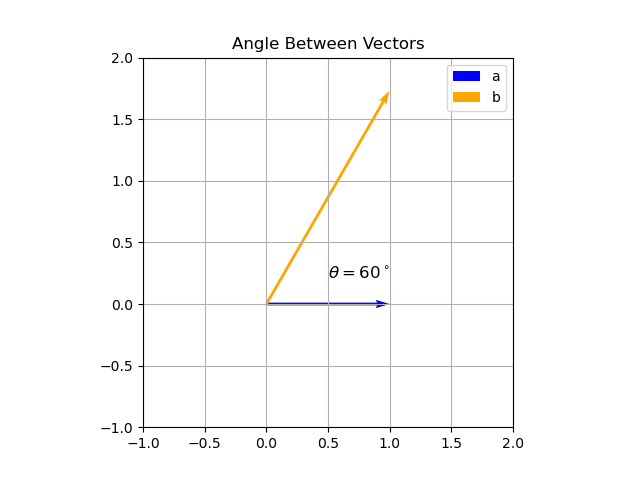
\includegraphics[width=0.7\linewidth]{../figs/Figure_1.png}
        \caption{}
        \label{fig:fig1}
    \end{figure}
\end{frame}

\end{document}
